\section{Diskussion}
\label{sec:Diskussion}

Der ermittelte Wert für $\frac{h}{e_0}$ beläuf sich auf $(4,66 \pm 0,58) \cdot 10^{-15} \si{\volt\second}$. Dies bedeutet eine Abweichung von 12,6\% vom Literaturwert von
$(4,14 \pm 0,58) \cdot 10^{-15} \si{\volt\second}$. 
\newline
Insgesamt entsprechen alle Ergebnisse den Erwartungen. Die Messung der roten Spektrallinie könnte hierbei noch den größten Einfluss auf die Abweichung zum Literaturwert
liefern, da der Spannungsbereich, der sich für die Messungen eignet, aufgrund der geringen maximalen Gegenspannung sehr klein ist. Die Spannungsschritte zwischen den
einzelnen Messungen des Photostroms wurden deshalb bei dieser Messung kleiner gewählt, als bei den anderen. Da es allerdings, aufgrund der Messapparatur für den Photostrom,
nicht möglich war, diesen beliebig genau abzulesen, wurden teilweise für mehrere Gegenspannungen die selben Stromstärken gemessen. Dies erklärt den deutlich
in \autoref{fig:rot} zu sehenden treppenartigen Verlauf der Messwerte.

\section{Anhang}
\label{sec:Anhang}

\begin{figure}[H]
    \centering
    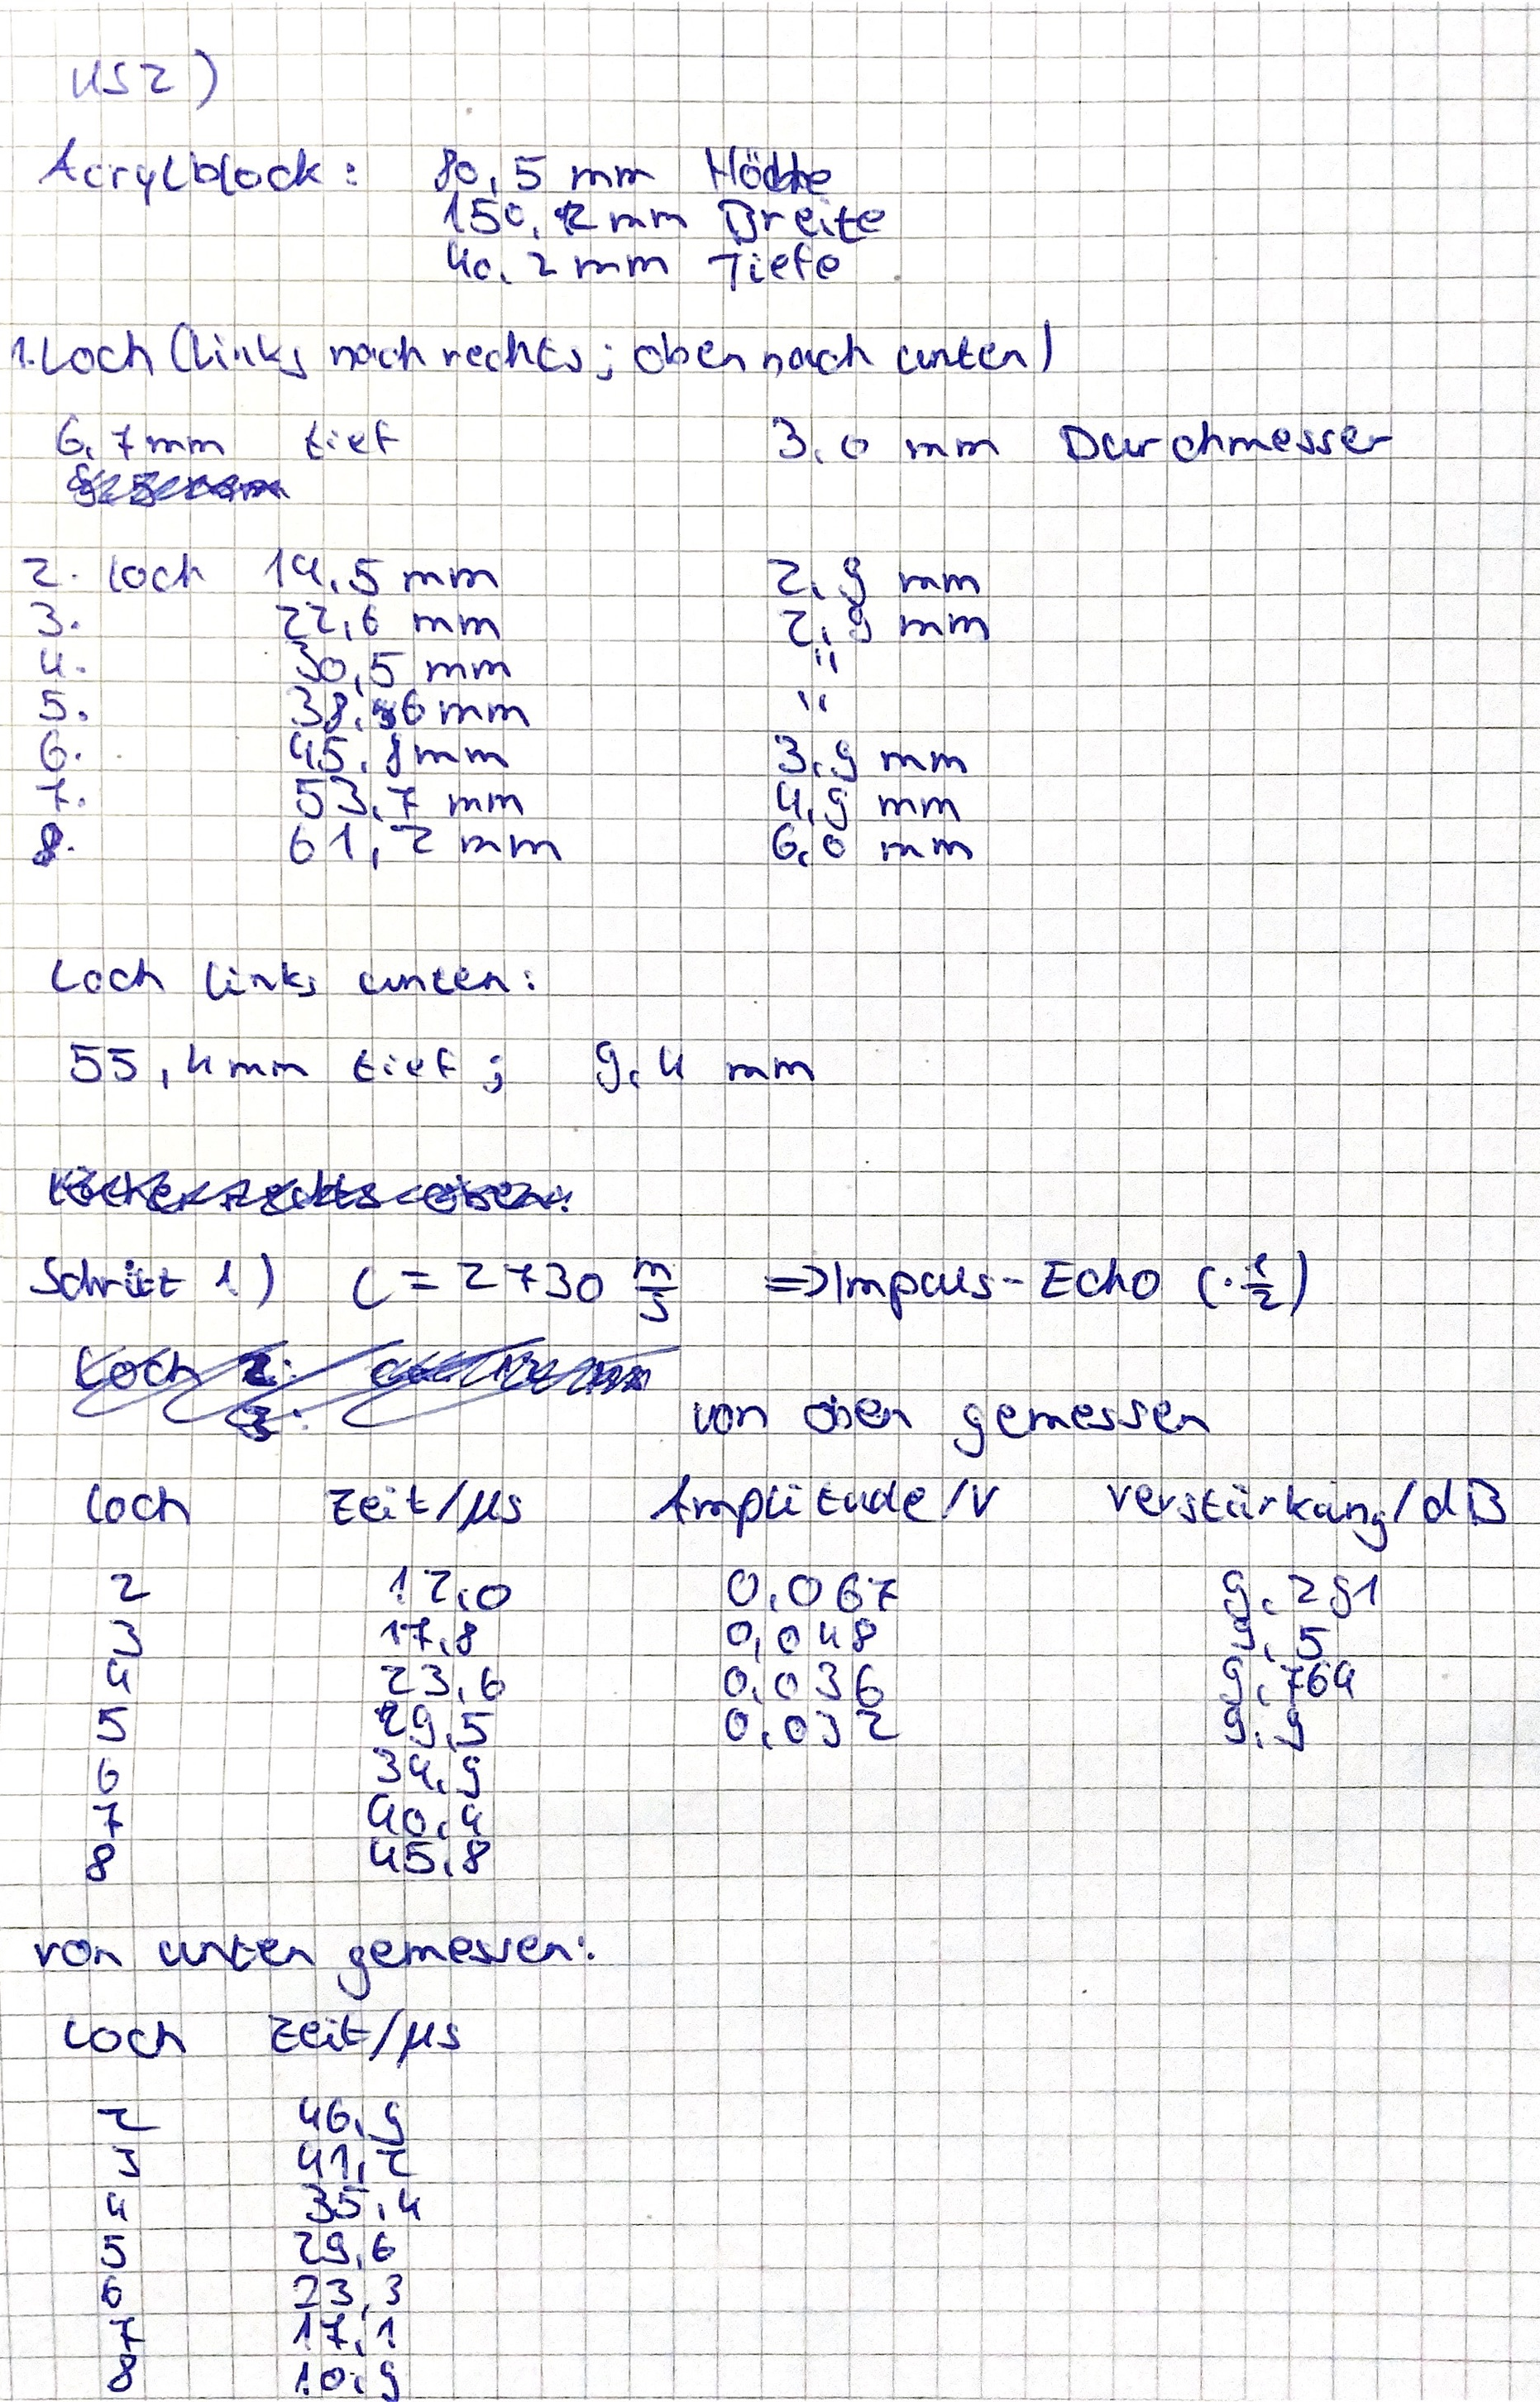
\includegraphics[width=0.75\textwidth]{data/origDaten1.jpg}
    \caption{Originale Messdaten des Versuches.}
    \label{fig:origData1}
\end{figure}
\begin{figure}[H]
    \centering
    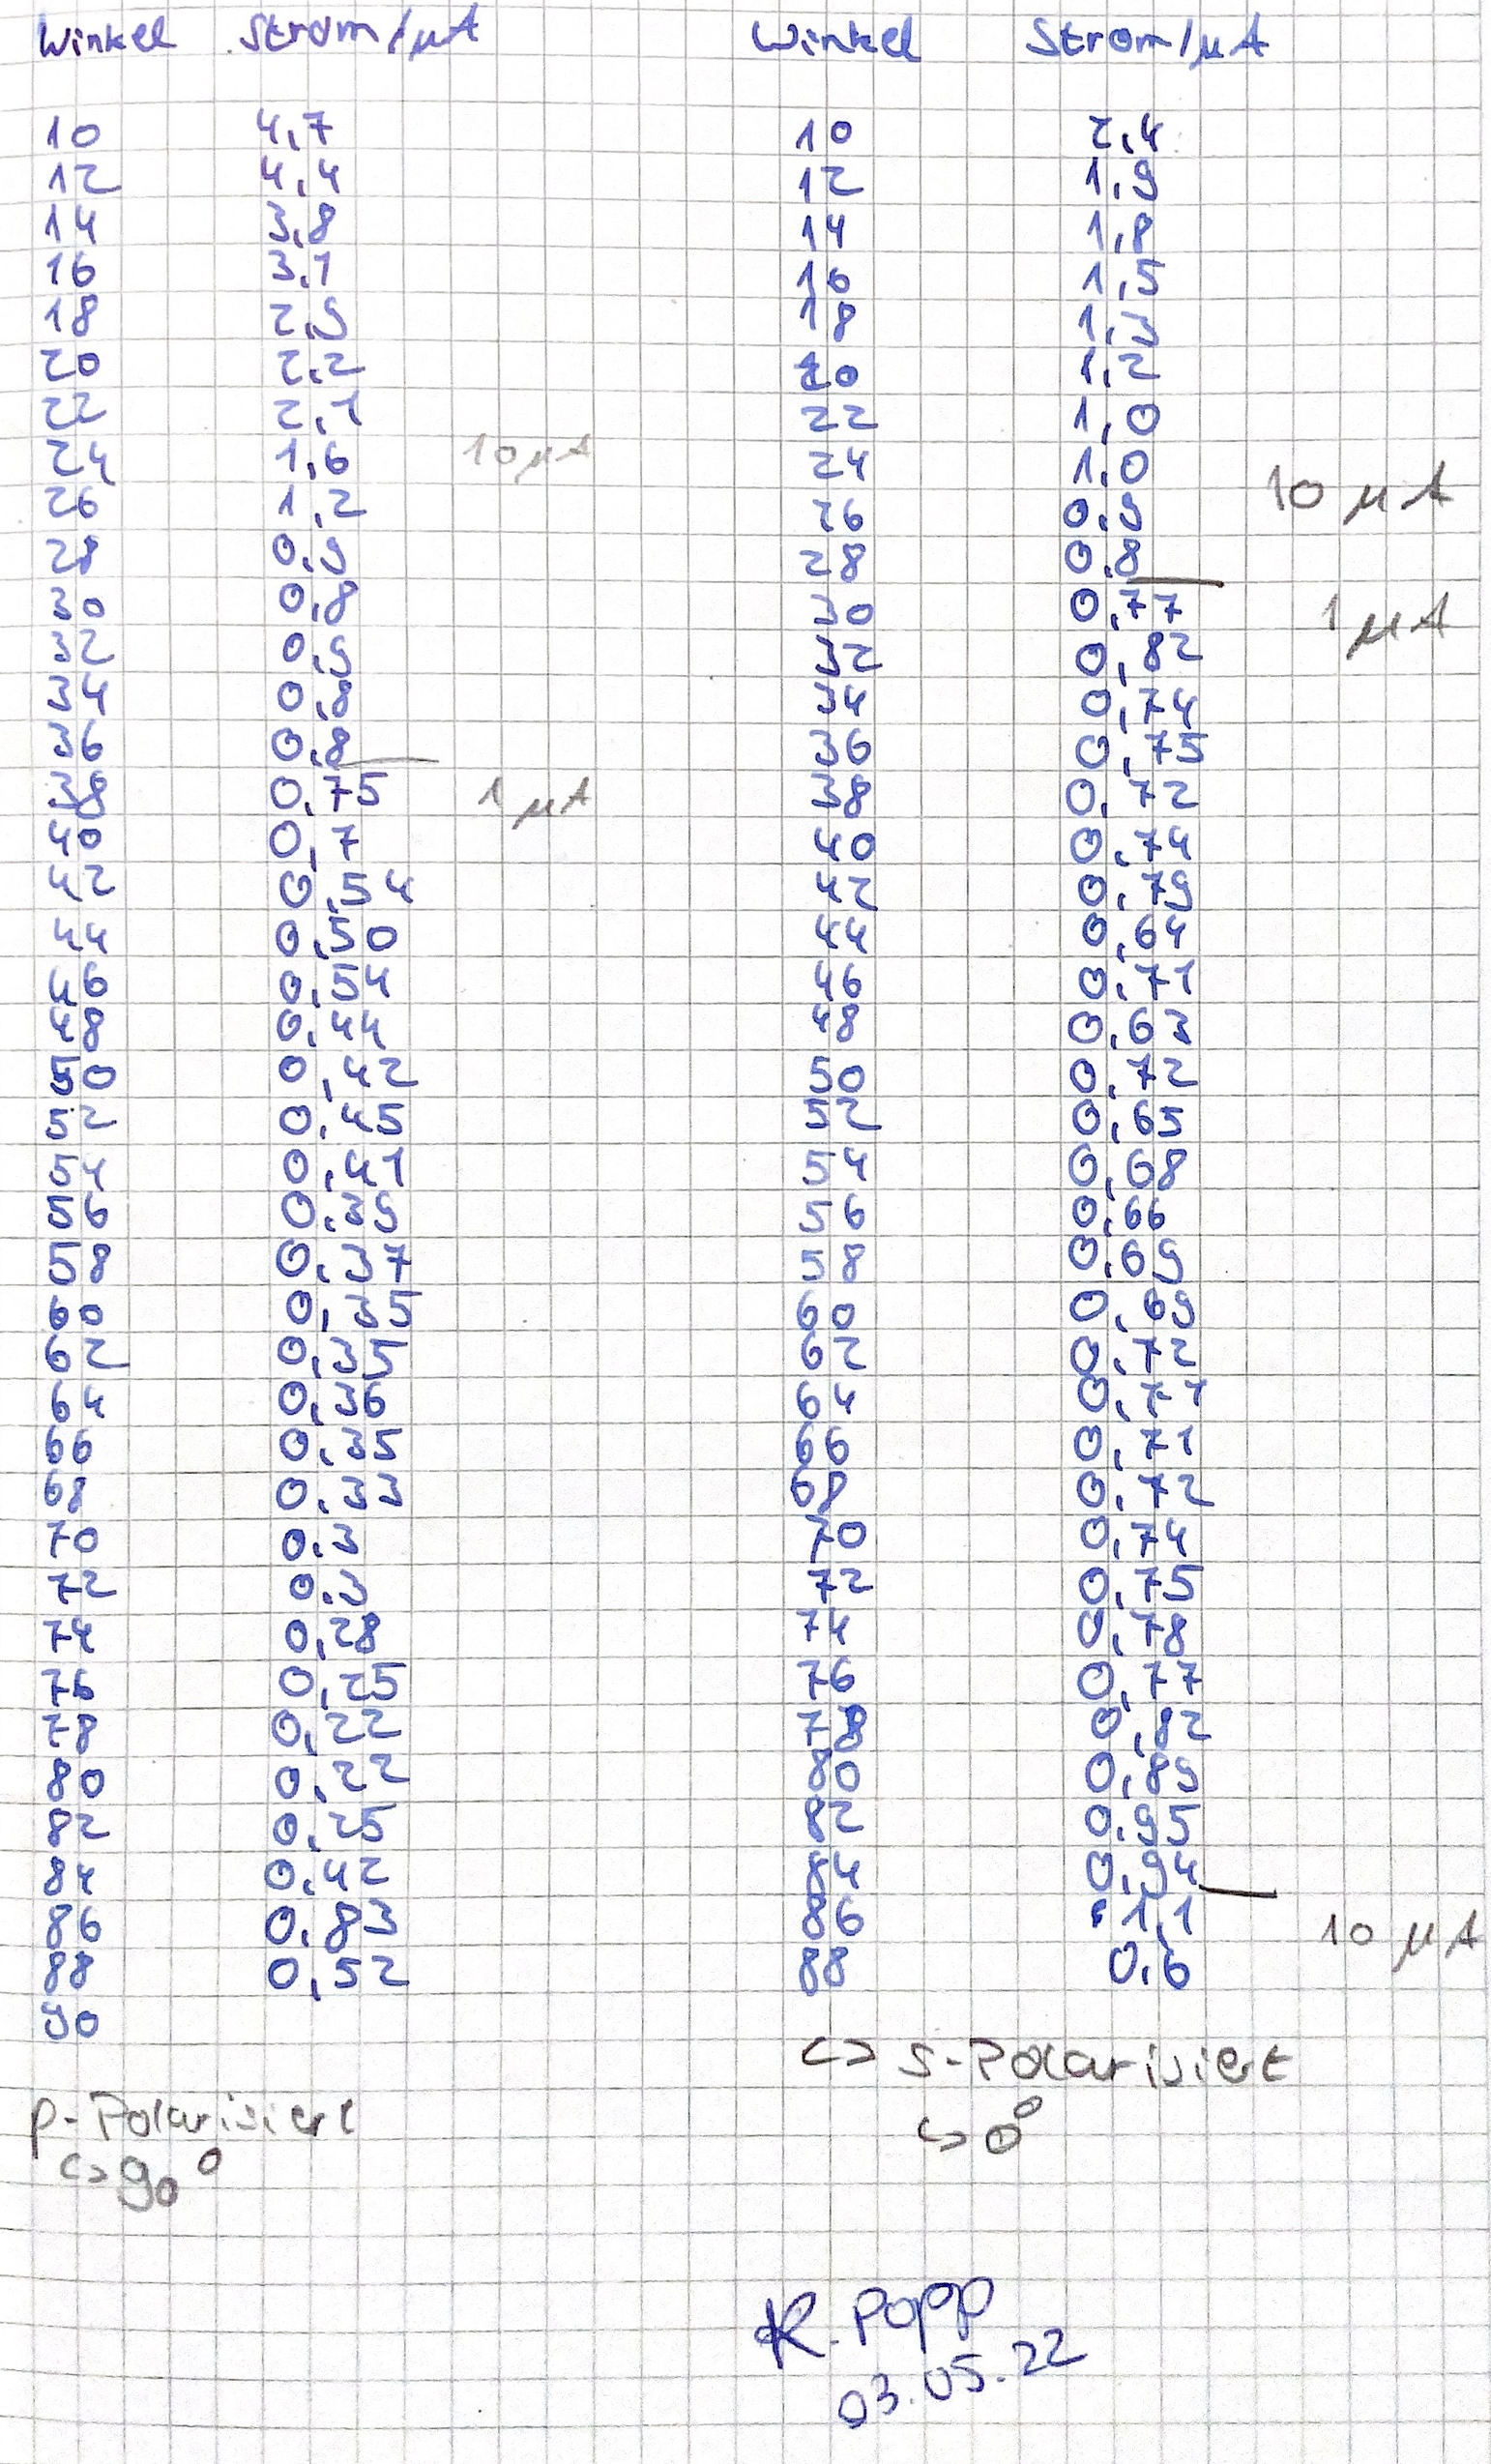
\includegraphics[width=0.75\textwidth]{data/origDaten2.jpg}
    \caption{Originale Messdaten des Versuches.}
    \label{fig:origData2}
\end{figure}
\begin{figure}[H]
    \centering
    \includegraphics[width=0.75\textwidth]{data/origDaten3.jpg}
    \caption{Originale Messdaten des Versuches.}
    \label{fig:origData3}
\end{figure}